\documentclass{article}
% Packages we need
\usepackage{amsmath}   % Math stuff - equations, etc.
\usepackage{amssymb}   % More math symbols
\usepackage{graphicx}  % For figures if we need them
\usepackage{hyperref}  % For linking and references
\usepackage{float}

\begin{document}

\section{What's a Box Kernel Anyway?}

I've been looking into different filtering methods lately, and thought I'd write up some notes on the box kernel (sometimes called the rectangular kernel or uniform filter). It's basically the simplest filter you can imagine - just a flat rectangular shape that averages things out.

Mathematically, we can write it as:
\[
h(t) =
\begin{cases}
\frac{1}{2T}, & \text{when } -T \le t \le T \\
0, & \text{everywhere else}
\end{cases}
\]

\subsection*{Main Characteristics}

\begin{itemize}
    \item The width is $2T$ overall (extends $T$ in each direction)
    
    \item Height is $\frac{1}{2T}$ - this weird-looking height is actually chosen so the total area equals 1
    
    \item It's normalized, meaning the area under the curve is exactly 1:
    \[
    \int_{-\infty}^{\infty} h(t) \, dt = \int_{-T}^{T} \frac{1}{2T} \, dt = 1
    \]
    
    This normalization turns out to be really important - it ensures that when we use the kernel for filtering, we don't artificially boost or reduce the signal's average value.
\end{itemize}

\subsection*{So What Does It Actually Do?}

When we use a box kernel, we're essentially taking a simple average over a window of time. For any point in our signal, we replace it with the average of all points within $T$ units to the left and right.

One thing to note - this is what signal processing folks call a \textbf{non-causal filter}. That means it needs both past AND future values of our signal. This works fine for offline processing (like photo editing), but isn't practical for real-time applications where we don't know future values yet. In those cases, we'd shift the box to only use past values.

\subsection*{Visual Picture}

If you plotted this function, you'd just see a rectangle (hence "box" kernel) of height $\frac{1}{2T}$ that starts at $-T$, stays flat until $+T$, then drops back to zero. Nothing fancy - just a box!

\begin{figure}
        \centering
        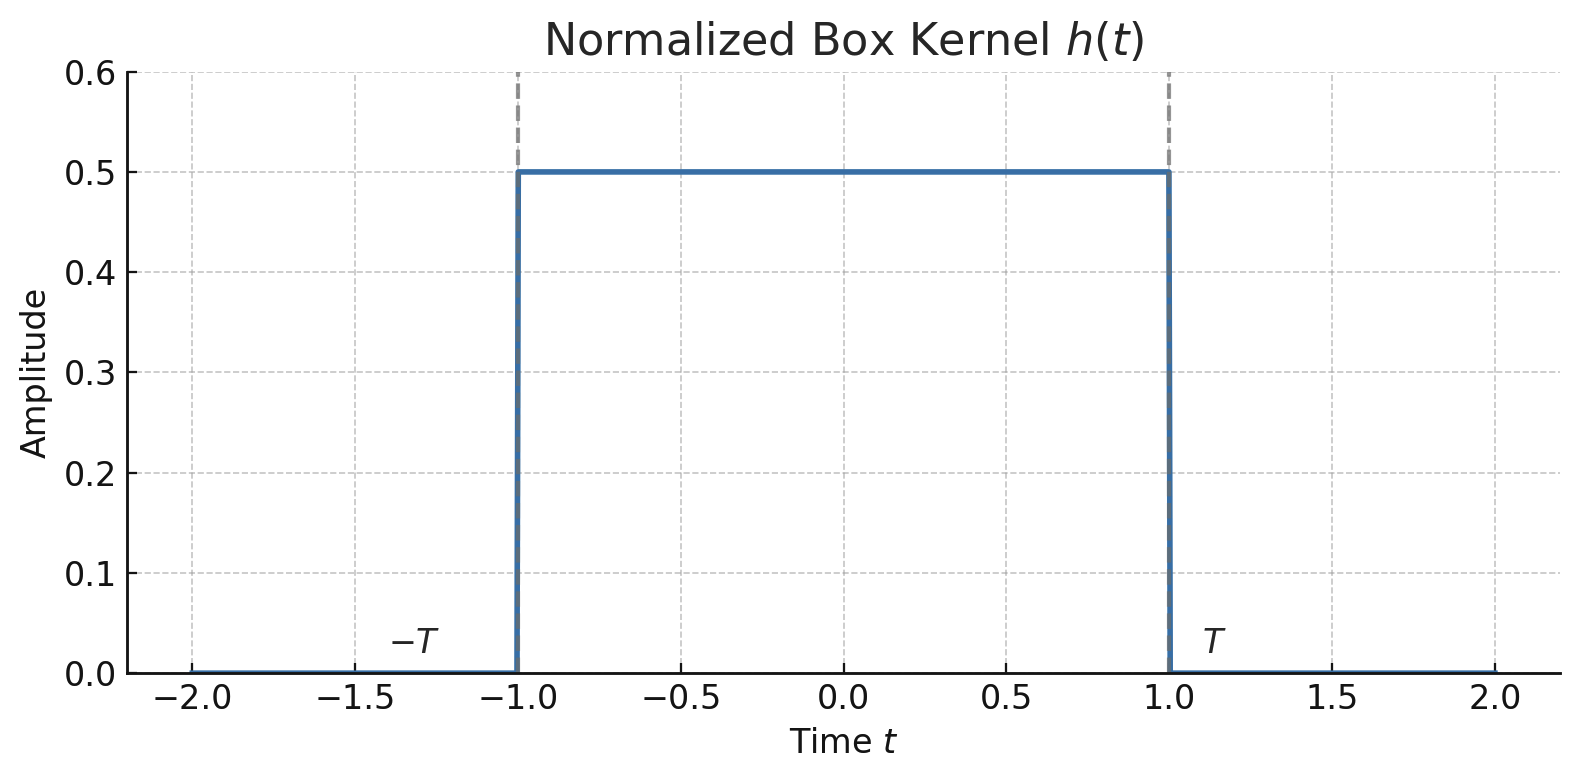
\includegraphics[width=1\linewidth]{figs/normal.png}
        \caption{Normalized Box Kernel: A rectangular function of height $\frac{1}{2T}$ spanning from $-T$ to $T$.}
        \label{fig:enter-label}
    \end{figure}
  
\section{Single Convolution with the Box Kernel}

In this section, we analyze the effect of a single convolution between a signal and a box (rectangular) kernel, considering both normalized and unnormalized versions of the kernel.

\subsection{Normalized Box Kernel}

The normalized box kernel is defined as:

\[
h(t) =
\begin{cases}
\frac{1}{2T}, & -T \le t \le T \\
0, & \text{otherwise}
\end{cases}
\]

The normalization ensures that the area under the kernel is 1, making it a proper averaging filter. We consider the convolution with a unit step function:

\[
f(t) = u(t) =
\begin{cases}
0, & t < 0 \\
1, & t \geq 0
\end{cases}
\]

The convolution is:

\[
y(t) = (f * h)(t) = \int_{-\infty}^{\infty} f(\tau) h(t - \tau) \, d\tau
\]

This results in a linear ramp from 0 to 1 over the interval \([-T, T]\), followed by a constant value of 1. The smoothing effect is evident as the sharp edge of the step function becomes a gradual transition.

\begin{figure}[H]
    \centering
    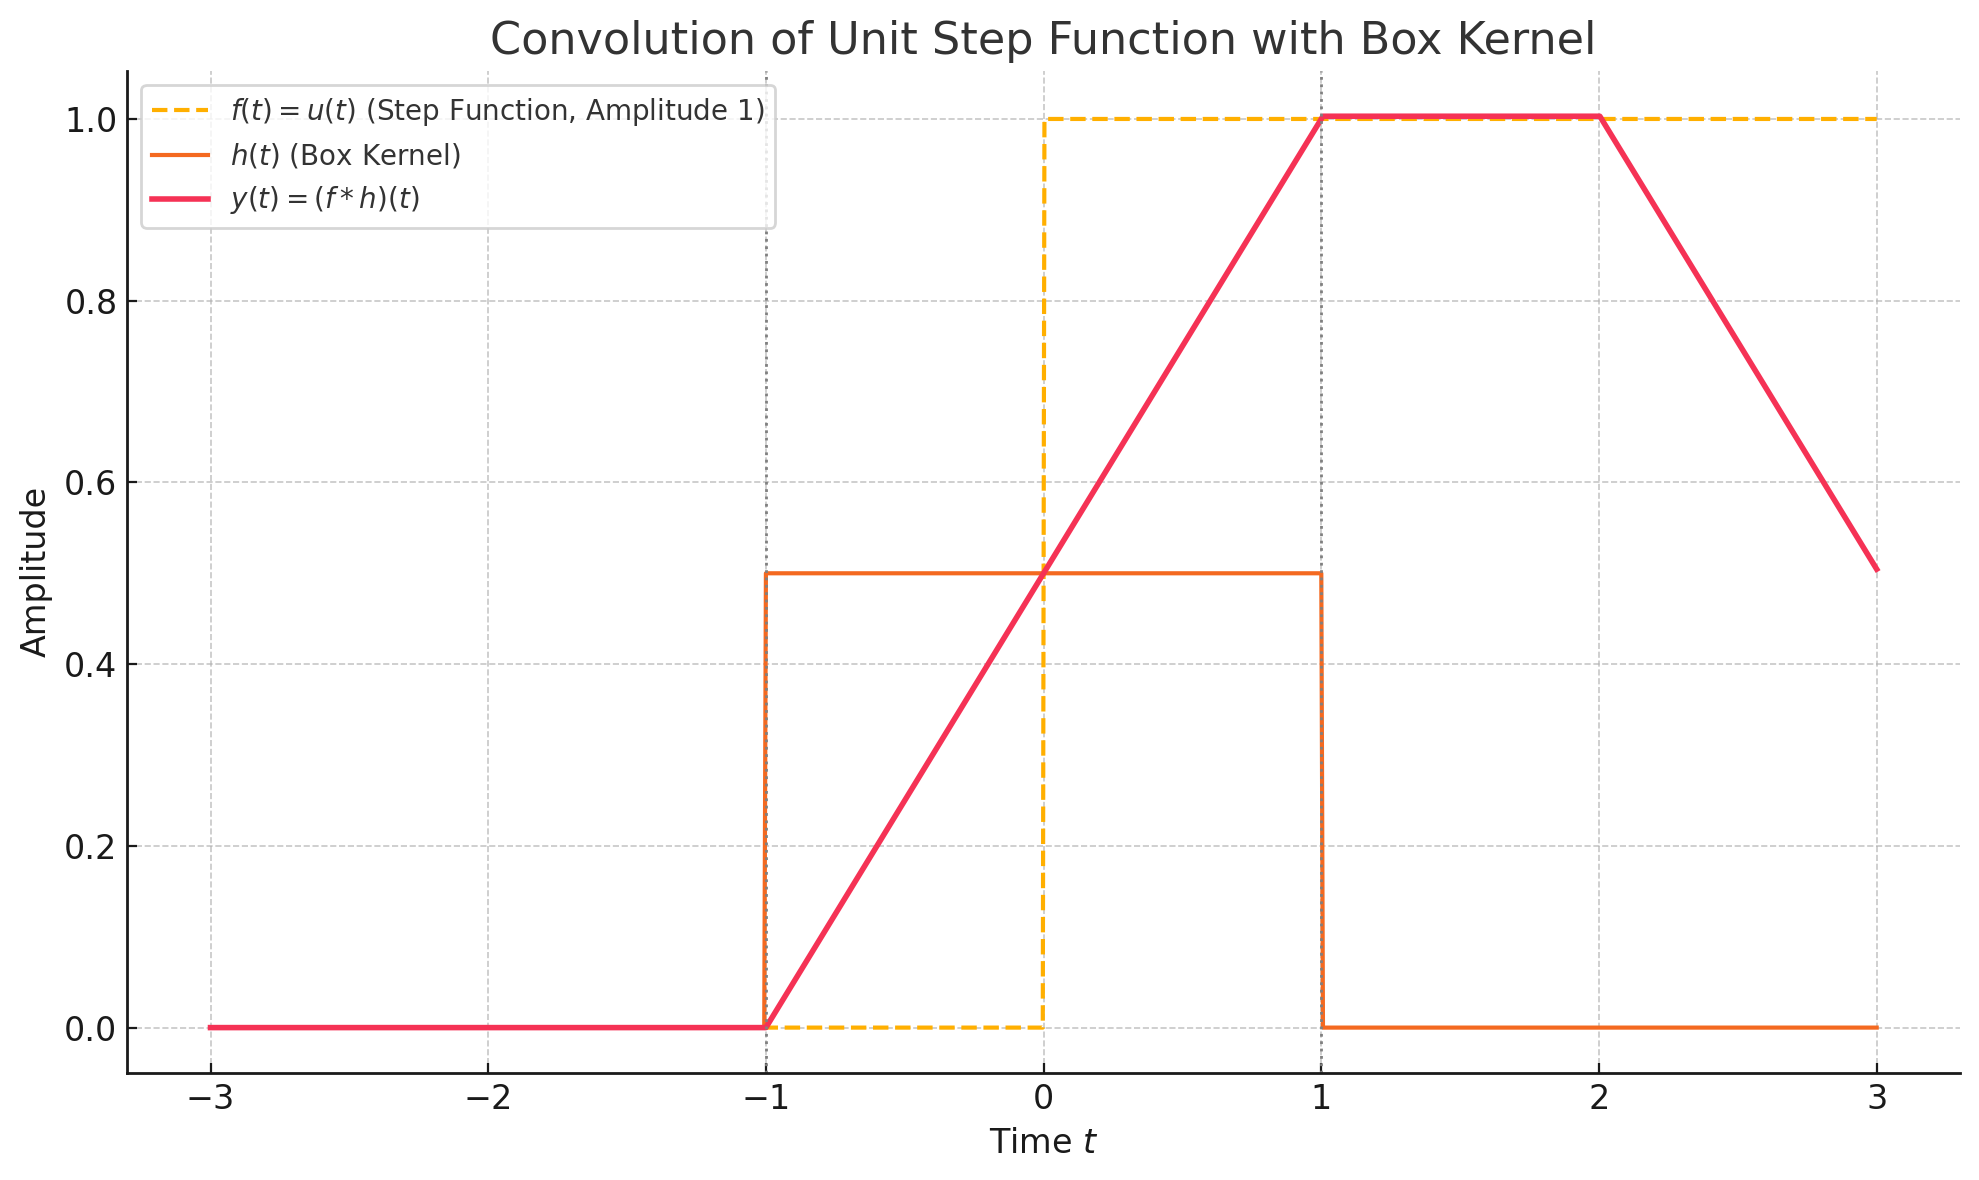
\includegraphics[width=0.9\linewidth]{figs/normalized.png}
\caption{Convolution of unit step function with normalized box kernel (height \(\frac{1}{2T}\))}
\end{figure}

\subsection{Unnormalized Box Kernel}

In this case, we define the box kernel with unit amplitude:

\[
h(t) =
\begin{cases}
1, & -T \le t \le T \\
0, & \text{otherwise}
\end{cases}
\]

This kernel does not preserve the average, but simply accumulates values across a flat window. The convolution with the same step function results in a ramp from 0 to \(2T\), after which the output remains constant.

\begin{figure}[H]
    \centering
    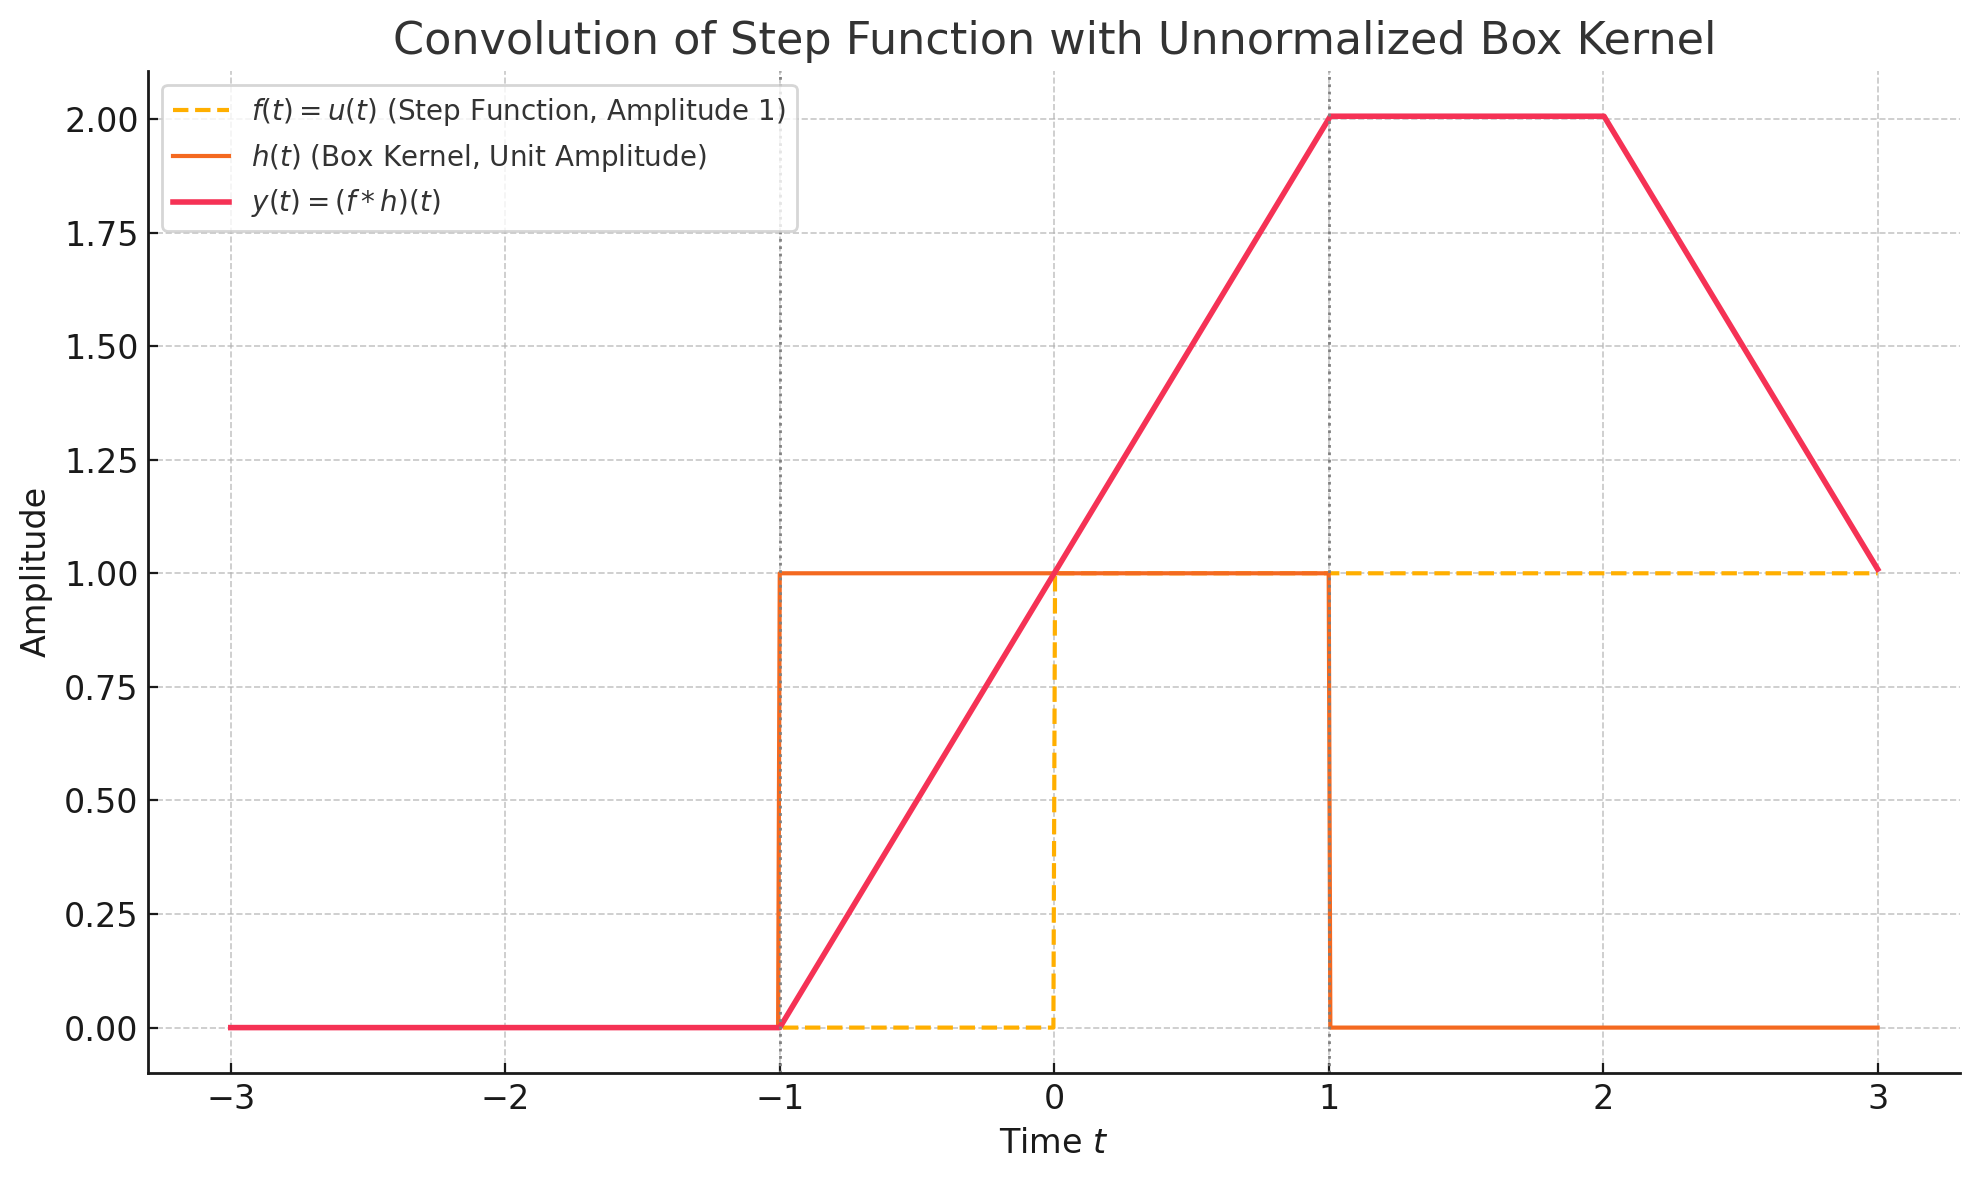
\includegraphics[width=1\linewidth]{figs/unnormalized_box.png}
\caption{Convolution of unit step function with unnormalized box kernel (height 1)}
\end{figure}

\subsection{Comparison and Interpretation}

\begin{itemize}
    \item The \textbf{normalized kernel} produces a smoothed version of the step function that transitions from 0 to 1.
    \item The \textbf{unnormalized kernel} produces a ramp that reaches \(2T\), since the full area under the kernel contributes to the accumulation.
\end{itemize}

This difference is crucial in applications: normalization is important when maintaining signal magnitude is required (e.g., in filtering or probability), whereas unnormalized kernels are useful when measuring cumulative effects.

\section{Repeated Convolution with the Box Kernel}

In this section, we investigate the result of repeatedly convolving a signal with the same box kernel. Repeated convolution involves applying the convolution operation multiple times, where the output of one convolution becomes the input for the next.

\subsection*{Mathematical Formulation}

Let \( f(t) \) be a signal, and let \( h(t) \) be the box kernel defined as:

\[
h(t) =
\begin{cases}
\frac{1}{2T}, & \text{for } -T \leq t \leq T \\
0, & \text{otherwise}
\end{cases}
\]

For the first convolution, we have:

\[
y_1(t) = (f * h)(t) = \int_{-\infty}^{\infty} f(\tau) h(t - \tau) \, d\tau
\]

For subsequent convolutions, the result of each convolution is treated as the input for the next:

\[
y_n(t) = (y_{n-1} * h)(t)
\]

Thus, the \( n \)-th convolution can be written as:

\[
y_n(t) = (f * h^n)(t)
\]

where \( h^n(t) \) represents the kernel \( h(t) \) convolved with itself \( n \) times.

\subsection*{Behavior of Repeated Convolution}

Each convolution with the box kernel has the effect of smoothing the signal further, reducing sharp transitions and spreading the signal over a wider interval. With each successive convolution, the result becomes progressively smoother and more spread out. The repeated averaging reduces high-frequency components, resulting in an increasingly gradual response.

As the number of convolutions increases, the signal approaches a smooth, more uniform shape, with less distinction between the original features of the signal.


 \section{Gaussian Approximation from Repeated Convolution}

In this section, we explore how repeated convolution of a signal with a box kernel leads to a Gaussian distribution. This behavior is a direct consequence of the \textbf{Central Limit Theorem (CLT)}. 

\subsection*{Central Limit Theorem (CLT) and Convolution}

The CLT states that the sum of a large number of independent random variables, each with the same distribution, approaches a Gaussian distribution as the number of variables increases. In the context of signal processing, this means that repeated convolution with the same kernel can produce a signal that approximates a Gaussian distribution.

The box kernel acts as an averaging filter, and when it is convolved with a signal multiple times, the resulting signal becomes increasingly smooth and more similar to a Gaussian function.

\subsection*{Gaussian Approximation}

As discussed in the previous section, the output of repeated convolutions with the box kernel \( h(t) \) can be written as:

\[
y_n(t) = (f * h^n)(t)
\]

With each convolution, the signal smooths out more, and after many iterations, the result approaches a Gaussian distribution. Specifically, the output \( y_n(t) \) converges to a Gaussian function with mean \( 0 \) and variance \( \sigma^2 \), where \( \sigma \) depends on the kernel width and the number of convolutions.

\[
y_n(t) \to \mathcal{N}(0, \sigma^2)
\]

The standard deviation \( \sigma \) increases with the number of convolutions, and the width of the Gaussian distribution becomes larger as more convolutions are applied.

\subsection*{Numerical Illustration}

We can observe the convergence to a Gaussian distribution by plotting the result of repeated convolutions. Initially, the signal will have sharp transitions and peaks. After several convolutions, the signal will become smoother and approach the shape of a Gaussian curve.

\begin{figure}[H]
\centering
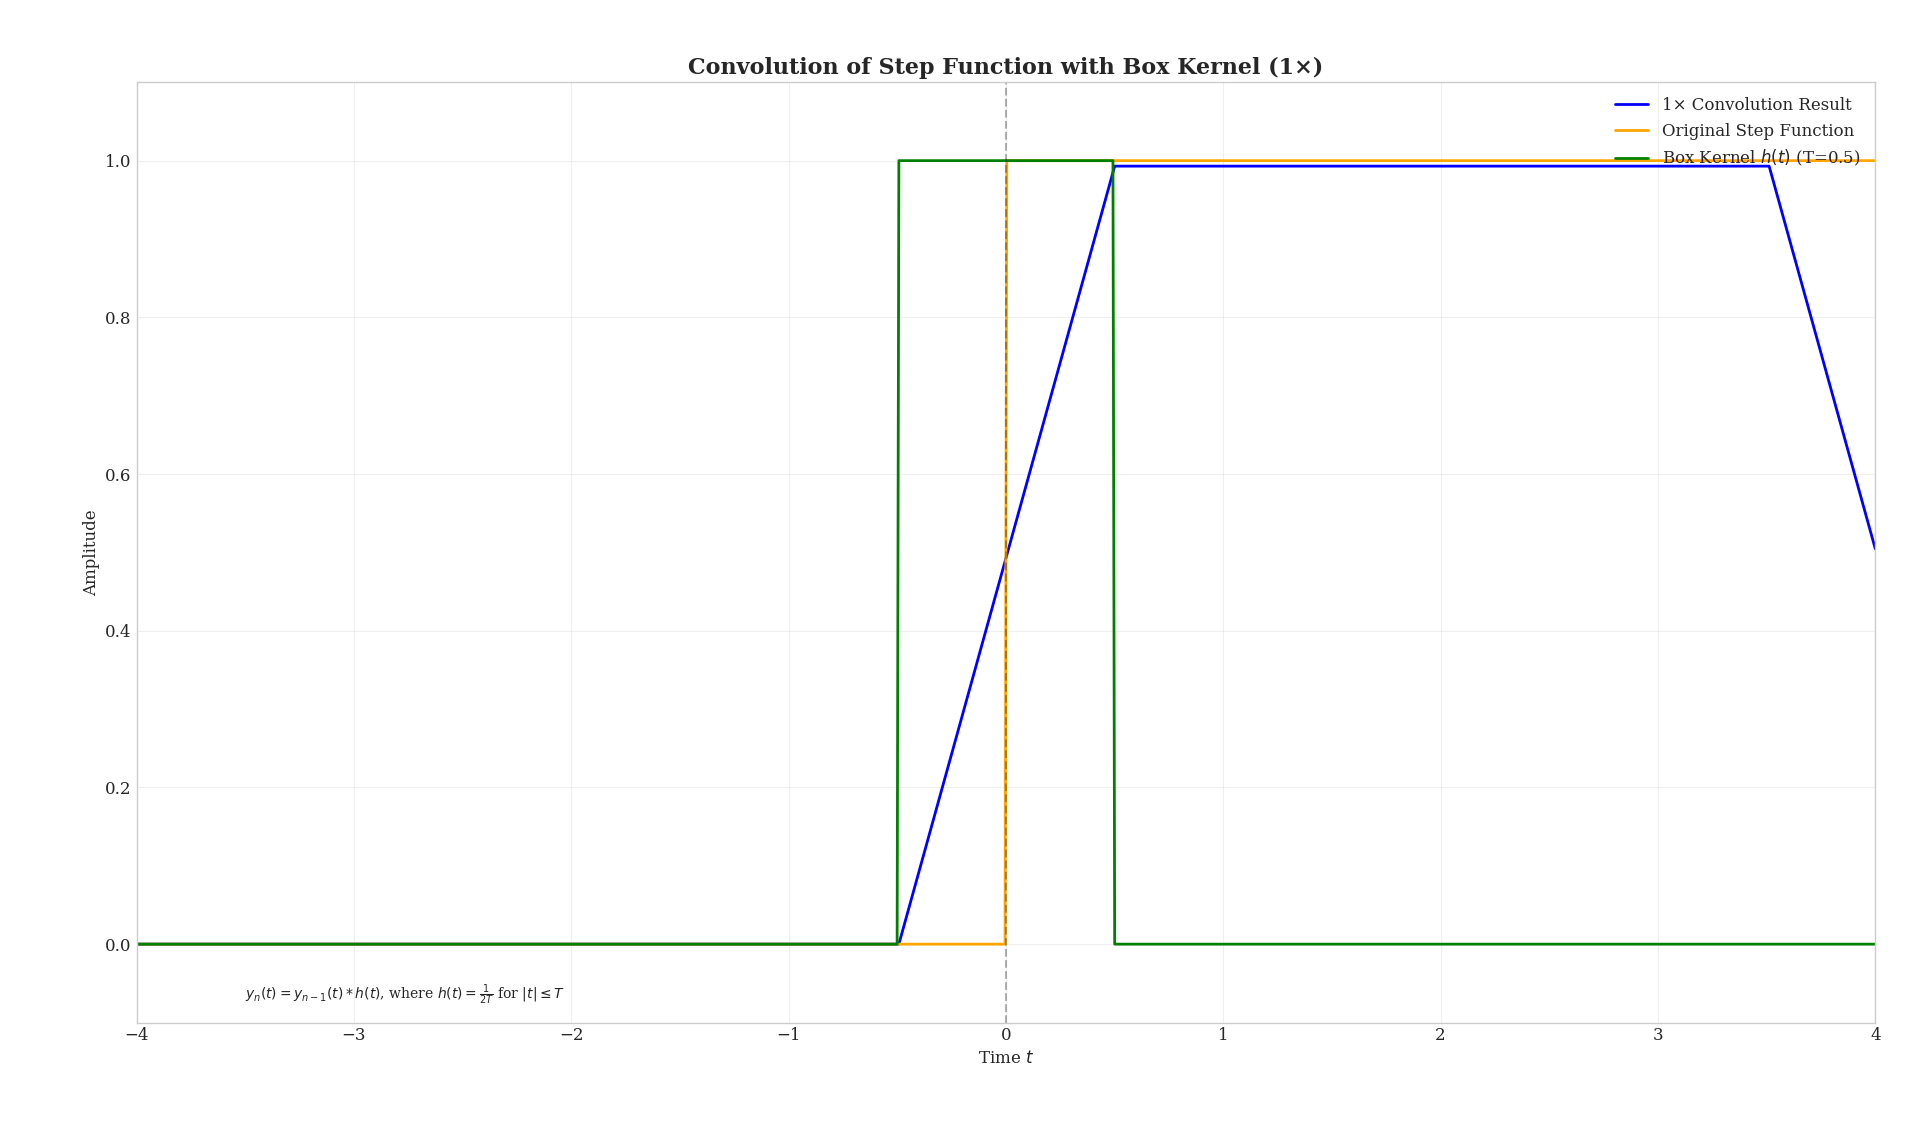
\includegraphics[width=1\textwidth]{figs/1_repeat.png}
\caption{Step Function Convolved Once with Box Kernel}
\end{figure}

\begin{figure}[H]
\centering
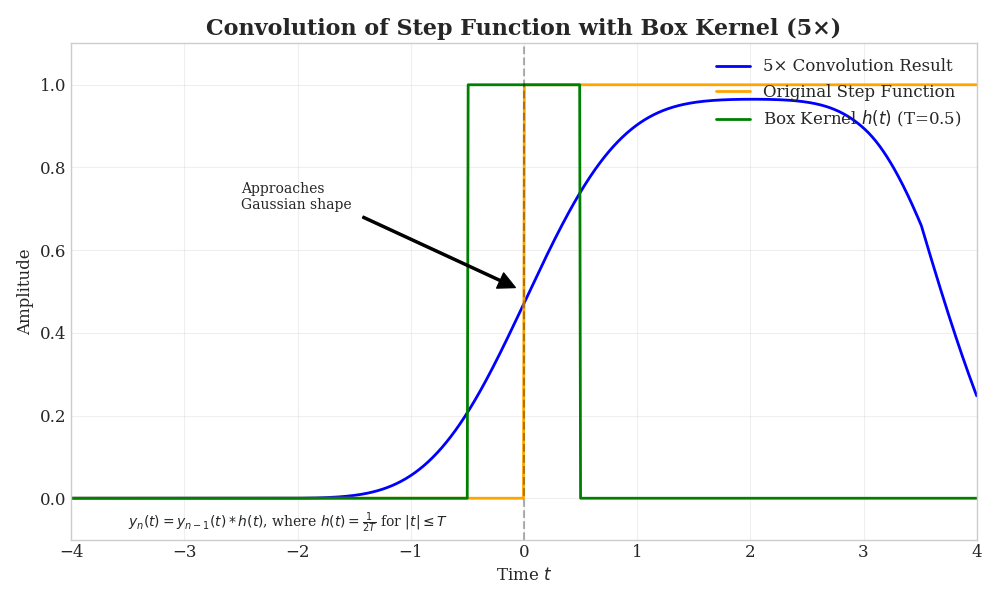
\includegraphics[width=1\textwidth]{figs/5_repeat.png}
\caption{Result of Five Consecutive Convolutions with Box Kernel}
\end{figure}

\begin{figure}[H]
\centering
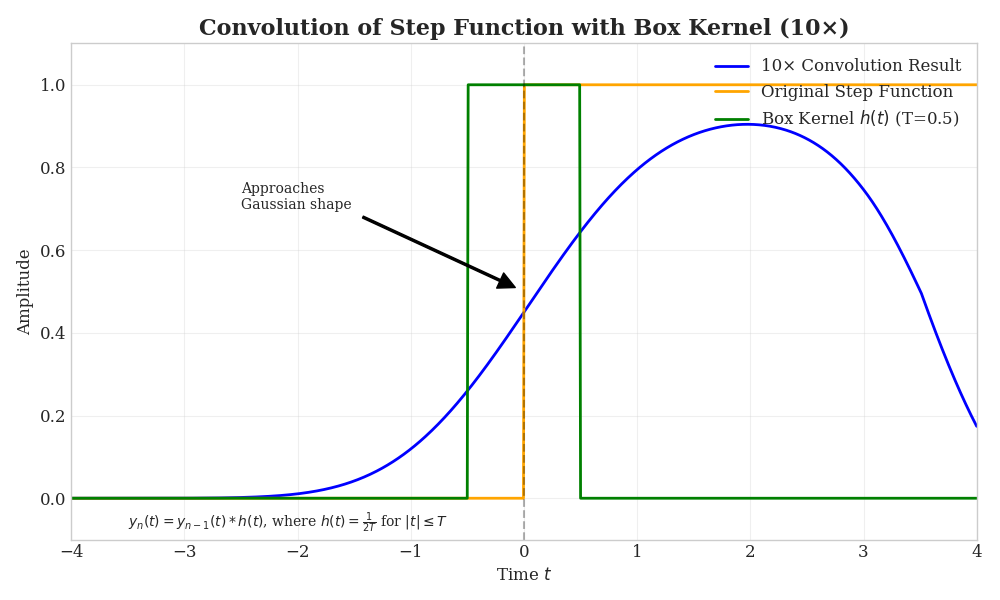
\includegraphics[width=1\textwidth]{figs/10_repeat.png}
\caption{Result of Ten Consecutive Convolutions with Box Kernel}
\end{figure}

\begin{figure}[H]
\centering
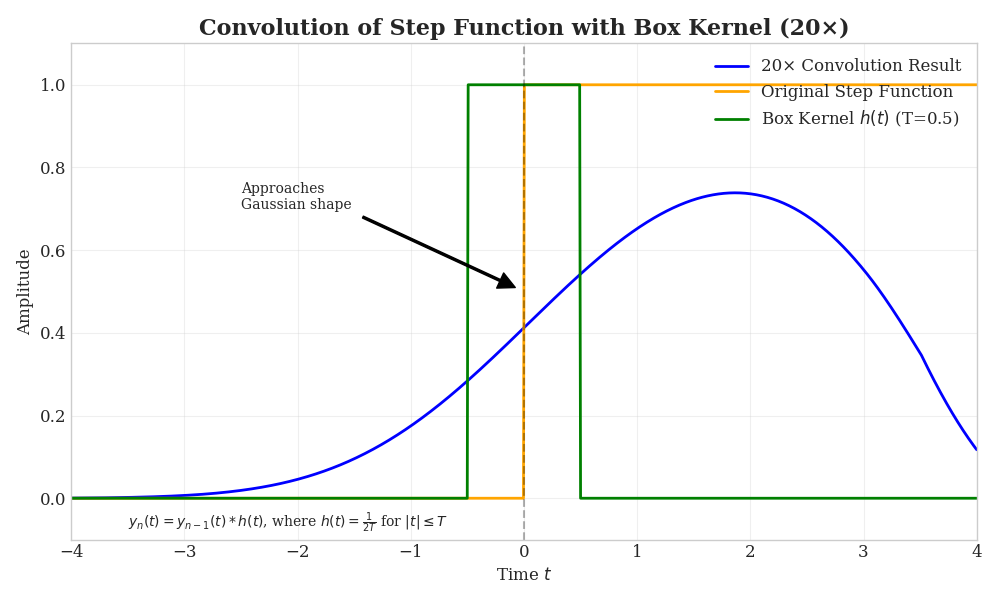
\includegraphics[width=1\textwidth]{figs/20_repeation.png}
\caption{Result of Twenty Consecutive Convolutions with Box Kernel}
\end{figure}

\subsection*{Conclusion}

Repeated convolution with a box (rectangular) kernel illustrates a fundamental principle from probability theory: the Central Limit Theorem (CLT). The CLT states that the sum (or average) of a large number of independent and identically distributed (i.i.d.) random variables—regardless of their original distribution—tends toward a Gaussian (normal) distribution as the number of terms increases.

In the context of signal processing, each convolution with a normalized box kernel can be interpreted as a smoothing operation that averages local values. Mathematically, this is analogous to summing independent uniform distributions (since the box kernel is uniform over its support). When the convolution is repeated multiple times, the result approximates the sum of multiple uniform distributions. According to the CLT, the shape of this sum converges to that of a Gaussian function as the number of repetitions increases.

Therefore, the repeated convolution of even a simple step function with a box kernel produces a progressively smoother output that increasingly resembles a Gaussian curve. This behavior is not just theoretical—it has practical importance in signal smoothing, noise reduction, and approximating Gaussian filters using simple kernels.

This convergence highlights the universality of the Gaussian distribution and the power of convolution as a tool in engineering and data analysis.

\end{document}
